\documentclass[journal = jpccck, manuscript = suppinfo]{achemso}
\setkeys{acs}{usetitle = true}

\usepackage{amsmath}
\usepackage{times}
\usepackage{booktabs}
\usepackage{mathptmx}
\usepackage{multirow}

\title{Thermal Transport is Influenced by Nanoparticle Morphology: A
  Molecular Dynamics Study}

\author{Suzanne M. Neidhart}
\author{J. Daniel Gezelter}
\email{gezelter@nd.edu}
\affiliation[University of Notre Dame]{251 Nieuwland Science Hall\\ 
Department of Chemistry and Biochemistry\\ 
University of Notre Dame\\ 
Notre Dame, Indiana 46556}
\phone{574-631-7595}

\keywords{}

\begin{document}

\subsection{System Details}
Both the nanoparticle and planar systems contain only gold atoms and
hexane molecules.  The composition of the planar systems can be found
in Table \ref{tab:facet} and the nanoparticle system details can be
found in Tables \ref{tab:spheres}, \ref{tab:icosahedra}, and \ref{tab:cubos}.

Planar systems were constructed with the exposed $(hkl)$ facets
directed normal to the positive and negative $z$-axis.  The simulation
cell dimensions were set by the facet, and the simulation box was
enlarged along the $z$ dimension to a fixed size of 100 \AA.  The
remaining space was filled with hexane molecules to a density of
0.6548 $\text{g cm}^{-3}$.

\begin{table}
\centering
\caption{Composition of the solvated planar facet systems and the
  physical extent of the gold slabs ($L_x$, $L_y$, and $L_z$). The
  hexane molecules occupy the remainder of a 100 \AA\ box (length
  measured along the $z$-axis). 
  \label{tab:facet}}
\begin{tabular}{ c|cccc| c }
\toprule
Facet & Au atoms & $L_x$ (\AA) &$L_y$ (\AA) & $L_z$ (\AA) & Hexane Molecules\\
\midrule
(111) &  972 & 25.915	& 29.888 & 18.952 & 284      \\
(110) & 1800 & 40.131	& 34.089 & 20.280 & 498      \\
(100) & 1008 & 24.322	& 24.382 & 26.422 & 200      \\
\bottomrule
\end{tabular}
\end{table}


\begin{table}
\centering
\caption{Composition of the solvated nanosphere simulations.
  \label{tab:spheres}}
\begin{tabular}{ c|cc }
\toprule
        & \multicolumn{2}{c}{Components}\\
Particle Radius (\AA) & Au atoms & Hexane Molecules \\
\midrule
 9.20 $\pm$ 0.28  & 249   &  2894      \\
14.30 $\pm$ 0.31  & 887   &  6304      \\
19.07 $\pm$ 0.28  & 1985  &  8555      \\ 
24.09 $\pm$ 0.32  & 3925  & 11576      \\
29.03 $\pm$ 0.29  & 6699  & 15376      \\
34.01 $\pm$ 0.32  & 10641 &  9235      \\
38.88 $\pm$ 0.31  & 15707 &  8056      \\
\bottomrule
\end{tabular}
\end{table}

\begin{table}
\centering
\caption{Composition of the solvated icosahedral nanoparticle simulations.  
  \label{tab:icosahedra}}
\begin{tabular}{ cc|cc }
\toprule
       &            & \multicolumn{2}{c}{Components}\\
$n$ shells & radius (\AA) & Au atoms & Hexane Molecules \\
\midrule
4  &  9.45 $\pm$ 0.15  &   309 &  2894      \\
5  & 11.75 $\pm$ 0.17  &   561 &  4320      \\
6  & 14.07 $\pm$ 0.19  &   923 &  6304      \\
7  & 16.39 $\pm$ 0.21  &  1415 &  7414      \\
8  & 18.71 $\pm$ 0.25  &  2057 &  8555      \\
9  & 21.04 $\pm$ 0.27  &  2869 &  8555      \\
10 & 23.36 $\pm$ 0.30  &  3871 & 11576      \\
11 & 25.69 $\pm$ 0.32  &  5083 & 11576      \\
12 & 28.02 $\pm$ 0.35  &  6525 & 11576      \\
13 & 30.35 $\pm$ 0.38  &  8217 &  7741      \\
14 & 32.67 $\pm$ 0.41  & 10178 &  9235      \\
15 & 35.00 $\pm$ 0.43  & 12430 & 10911      \\
16 & 37.33 $\pm$ 0.66  & 14993 & 11576      \\
\bottomrule
\end{tabular}
\end{table}

\begin{table}
\centering
\caption{Composition of the solvated cuboctahedral nanoparticle simulations.
  \label{tab:cubos}}
\begin{tabular}{ c|cc }
\toprule
        & \multicolumn{2}{c}{Components}\\
 radius(\AA)      & Au atoms & Hexane Molecules \\
\midrule
 7.41 $\pm$ 0.35  &   147 & 11360      \\
10.16 $\pm$ 0.53  &   309 &  3387      \\
12.15 $\pm$ 0.50  &   561 &  5888      \\
14.98 $\pm$ 0.69  &   923 &  7414      \\
16.93 $\pm$ 0.65  &  1415 &  9440      \\
19.80 $\pm$ 0.85  &  2057 &  9380      \\
21.73 $\pm$ 0.82  &  2869 & 10317      \\
24.13 $\pm$ 0.90  &  3871 & 14185      \\
26.53 $\pm$ 0.99  &  5083 & 19585      \\
31.34 $\pm$ 1.15  &  8217 & 12626      \\
36.15 $\pm$ 1.32  & 12431 & 17457     \\
\bottomrule
\end{tabular}
\end{table}

For this work, gold -- gold interactions are calculated using the
quantum Sutton-Chen (QSC) model.\cite{Qi:1999ph} The hexane solvent is
described by the TraPPE united atom (UA)
model.\cite{TraPPE-UA.alkanes} The bonds in TraPPE-UA are rigid, but
here the bonds are made flexible using harmonic force constants
borrowed from OPLS-AA for intra-molecular sites closer than 3
bonds.\cite{Jorgensen98a} The interactions between Au atoms and atoms
on the hexane molecules were fit to a pairwise Lennard-Jones
potentials based on a study by Hautman and Klein for Au(111)
surfaces.\cite{hautman:4994} Details of the interaction potentials are
identical to previous work on heat transport for thiolate-protected
gold nanospheres.\cite{Stocker2016}

\subsection{Surface Atom Undercoordination}
In Table \ref{tab:undercoord}, we provide the surface density of
undercoordinated atoms for a set of ideal geometries. The population
density for the sphere systems in the large radius limit are taken by
averaging the surface densities for ideal gold nanospheres with radii
of 95--100 \AA.  For other FCC-based nanoparticles, it is relatively
simple to convert these surface densities using the lattice constant
of gold, $\ell = 4.08 \text{~\AA}$.

Planar facets have a fixed population density based on the number of
exposed undercoordinated atoms and the physical dimensions of the
exposed facet area in terms of the lattice constant.
\begin{figure}[!htb]
	\includegraphics[width=5in]{figures/facets-cn.pdf}
	\caption{Locations of undercoordinated atoms on common gold
          facets. The dark gold atoms indicate atoms of a particular
          coordination number, cyan atoms denote the first nearest
          neighbors of these atoms, and the partially transparent
          lattice illustrates the location of the atoms in the larger
          gold structure. (111) surfaces (lower left) display atoms
          with CN=9, while (100) surfaces (upper left) display atoms
          with CN=8, and (110) surfaces present surface atoms with
          CN=7 and buried atoms with CN=11. }
	\label{fig:facets-cn}
\end{figure}


In an ideal icosahedral nanoparticle with $n$ shells, the surface
population density is computed using the number of vertex, edge, and
face atoms,
\begin{align}
n_\text{vertex} & = 12, \\
n_\text{edge} & = 30 (n -1), \\
n_\text{face} & = 10 n^2 - 30 n + 20.
\end{align}  
The number of shells, $n$, is also directly related to the particle
edge length ($a$), radius ($r$), and surface area ($A$) of the
icosahedral particle,
\begin{align}
a & = \ell~n \\
r & = \frac{\ell~n~\sqrt{10+2\sqrt{5}}}{4} \\
A & =  \ell^2~n^2~ 5 \sqrt{3}
\end{align}
where $\ell$ is the lattice constant.

For ideal cuboctahedra, the edge length ($a$) can be used to determine
surface areas for the eight triangular (111) faces and six square
(100) faces,
\begin{align}
A_\mathrm{(111)} &= 2 \sqrt{3} a^2 \\
A_\mathrm{(100)} &= 6 a^2 
\end{align}
In addition, cuboctahedra have twenty-four edges (CN = 7, length =
$a$), and twelve vertices (CN = 5).  An approximate radius of the
cuboctahedral particles can be found by averaging the diameter between
parallel square faces and parallel triangular faces,
\begin{equation}
r  = \frac{a}{2} \left(\frac{\sqrt{2}}{2} + \frac{\sqrt{6}}{3}\right) 
\label{r_ave}
\end{equation} 
Tab. \ref{tab:undercoord}.  Surface densities of the CN=9 and CN=8
sites are computed using the fraction of total surface area in each of
the (111) and (100) facets, respectively.  For small particles, the
edge atoms (CN=7) can dominate, but for larger particles, the ratio of
CN=8 and CN=9 atoms is constant.  
\begin{table}
\centering
\caption{Surface densities $(\text{\AA}^{-2})$ of undercoordinated
  atoms in ideal geometries. $\ell~(\text{\AA})$ is the
  lattice constant of the underlying FCC lattice.  The spheres and
  cuboctahedra are calculated using a gold FCC lattice with $\ell = 4.08
  \text{~\AA}$.  For cuboctahedral particles, the radius ($r$) is computed
  using Eq. \eqref{r_ave}.
  \label{tab:undercoord}}
\begin{tabular}{ c|cccc }
\toprule
\multirow{2}{*}{surface} & \multicolumn{4}{c}{Coordination Number}\\
        & 6 & 7 & 8 & 9 \\
 \midrule
(111)      & 0 & 0     & 0     & $\frac{4 \sqrt{3}}{3 \ell^2}$ \\
(100)      & 0 & 0     & $\frac{2}{\ell^2}$ & 0     \\
(110)      & 0 & $\frac{\sqrt{2}}{\ell^2}$ & 0     & 0     \\  
 \midrule
Spheres (large $r$ limit)    & 0.021 & 0.025 & 0.021 & 0.032\\ \\
Icosahedra ($n$ shells)  & $\frac{8\sqrt{3}}{5\ell^2n^2}$  &  0 &
 $\frac{4\sqrt{3}(n-1)}{\ell^2n^2}$ &
 $\frac{4(n - 1)}{\sqrt{3}\ell^2 n}$ \\ \\
Cuboctahedra & 0 & $\frac{1}{r\ell} \left(\frac{3\sqrt{2} + 2\sqrt{6}}{3+\sqrt{3}}\right)$ & $\frac{6}{(3+\sqrt{3})\ell^2}$ & $\frac{4}{(3+\sqrt{3})\ell^2}$\\ \\
\bottomrule
\end{tabular}
\end{table}

 
%%%%%%%%%%%%%%%%%%%%%%%%%%%%%%%%%%%%%%%
%%% Vibrational DOS %%%
%%%%%%%%%%%%%%%%%%%%%%%%%%%%%%%%%%%%%%%
\subsection{Vibrational Density of States}

The vibrational density of states (VDOS) projected normal to the
interface were calculated for the gold atoms and the interfacial
solvent within 5 \AA\ of the gold particle.  These are plotted in
Fig. \ref{fig:all-spect}.  While the solvent VDOS in the icosahedral
and spherical systems shows only small changes as a function of
particle size, the solvent in the cuboctahedral systems appears to
shift to lower frequencies with increasing particle radius.  The gold
VDOS in all systems displays a shift from the low frequency peak,
$70 \mathrm{~cm}^{-1}$, to a peak at $125 \mathrm{~cm}^{-1}$ as the
particle radii increases and there is a significant difference between
the two FCC structures and the icosahedra spectra.  The FCC structures
increase in intensity at $125 \mathrm{~cm}^{-1}$ with increasing
particle radius, while the icosahedra VDOS shows a shift in population
from low frequencies to the higher frequency peak.  Note that the gold
shown in Fig. \ref{fig:all-spect} includes all layers of the
particles.

\begin{figure}[!htb]
	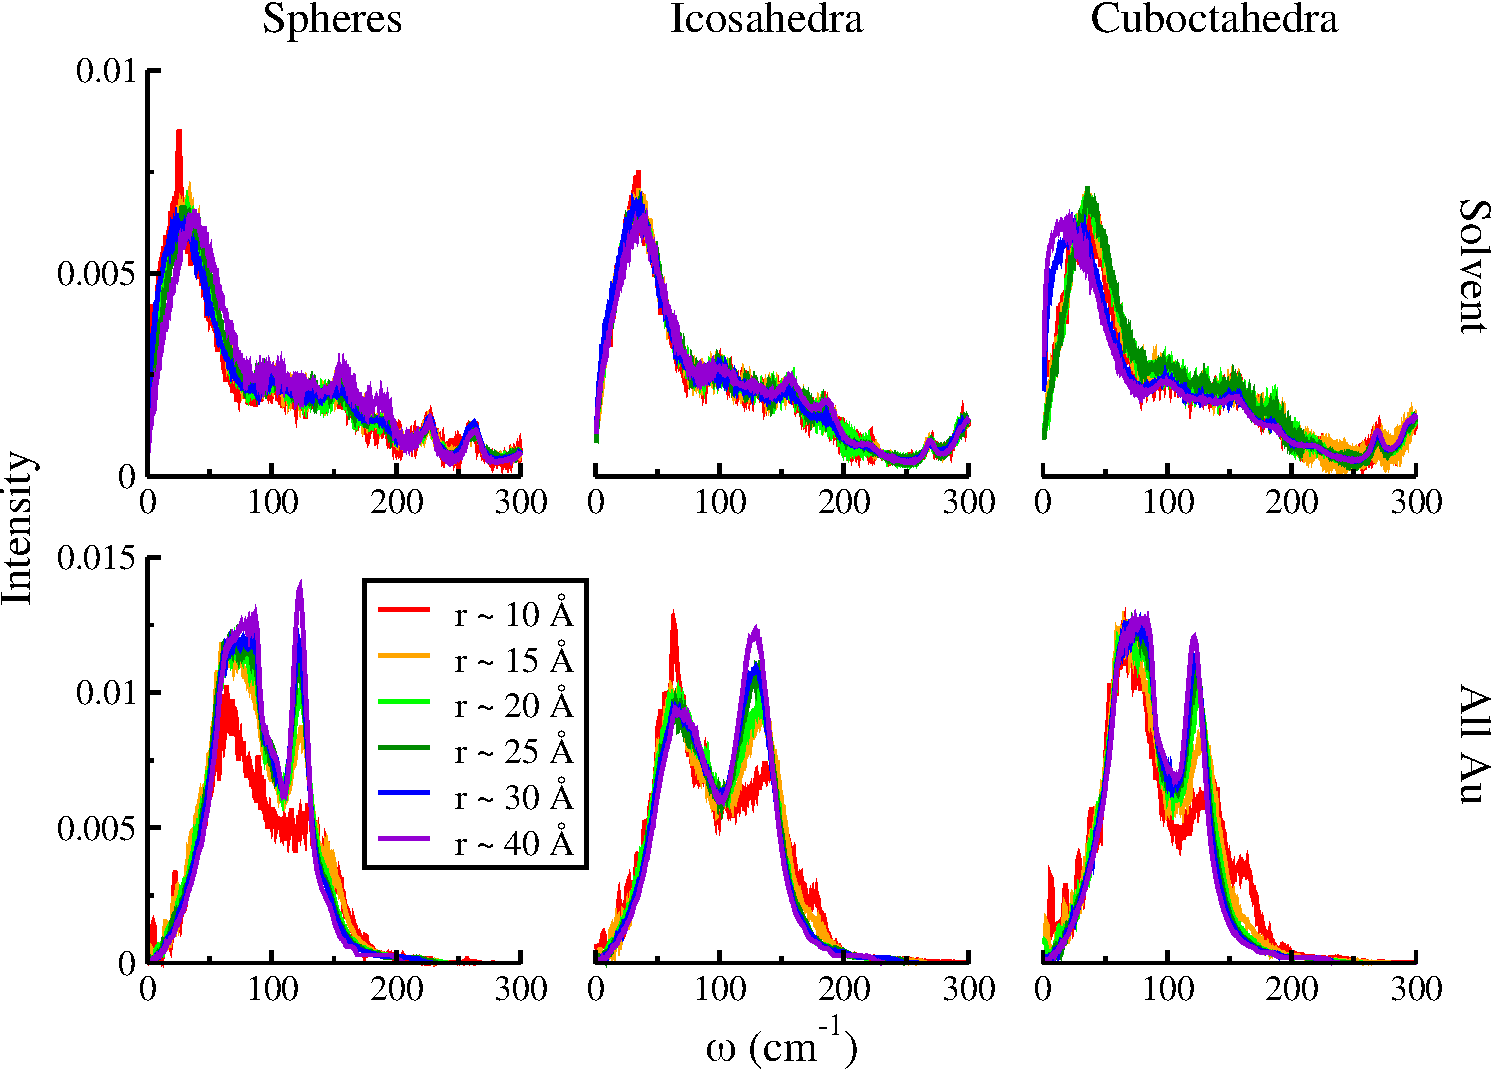
\includegraphics[width=5in]{figures/all-spect.pdf}
	\caption{The normalized low frequency density of states (DOS)
          of the interfacial solvent and the gold particle for the
          icosahedral and spherical systems. }
	\label{fig:all-spect}
\end{figure}

For individual coordination environments, it is possible isolate the
vibrational density of states from atoms on flat facets and the edge
atoms of icosahedra. The VDOS functions are shown in
Fig. \ref{fig:cn-spect}. The flat (111) and (100) facets provide
samples of 9- and 8-coordinated surface atoms, respectively, while the
(110) surface provides 7- and 11-coordinated atoms from the exposed
and subsurface layers. Sampling of 6-coordinated atoms comes from the
vertices of the stable icosahedra.  Note that during simulations, the
coordination environments change dynamically, so this should be
regarded only as an approximate picture of the vibrational
contributions from these coordination environments.

\begin{figure}[!htb]
  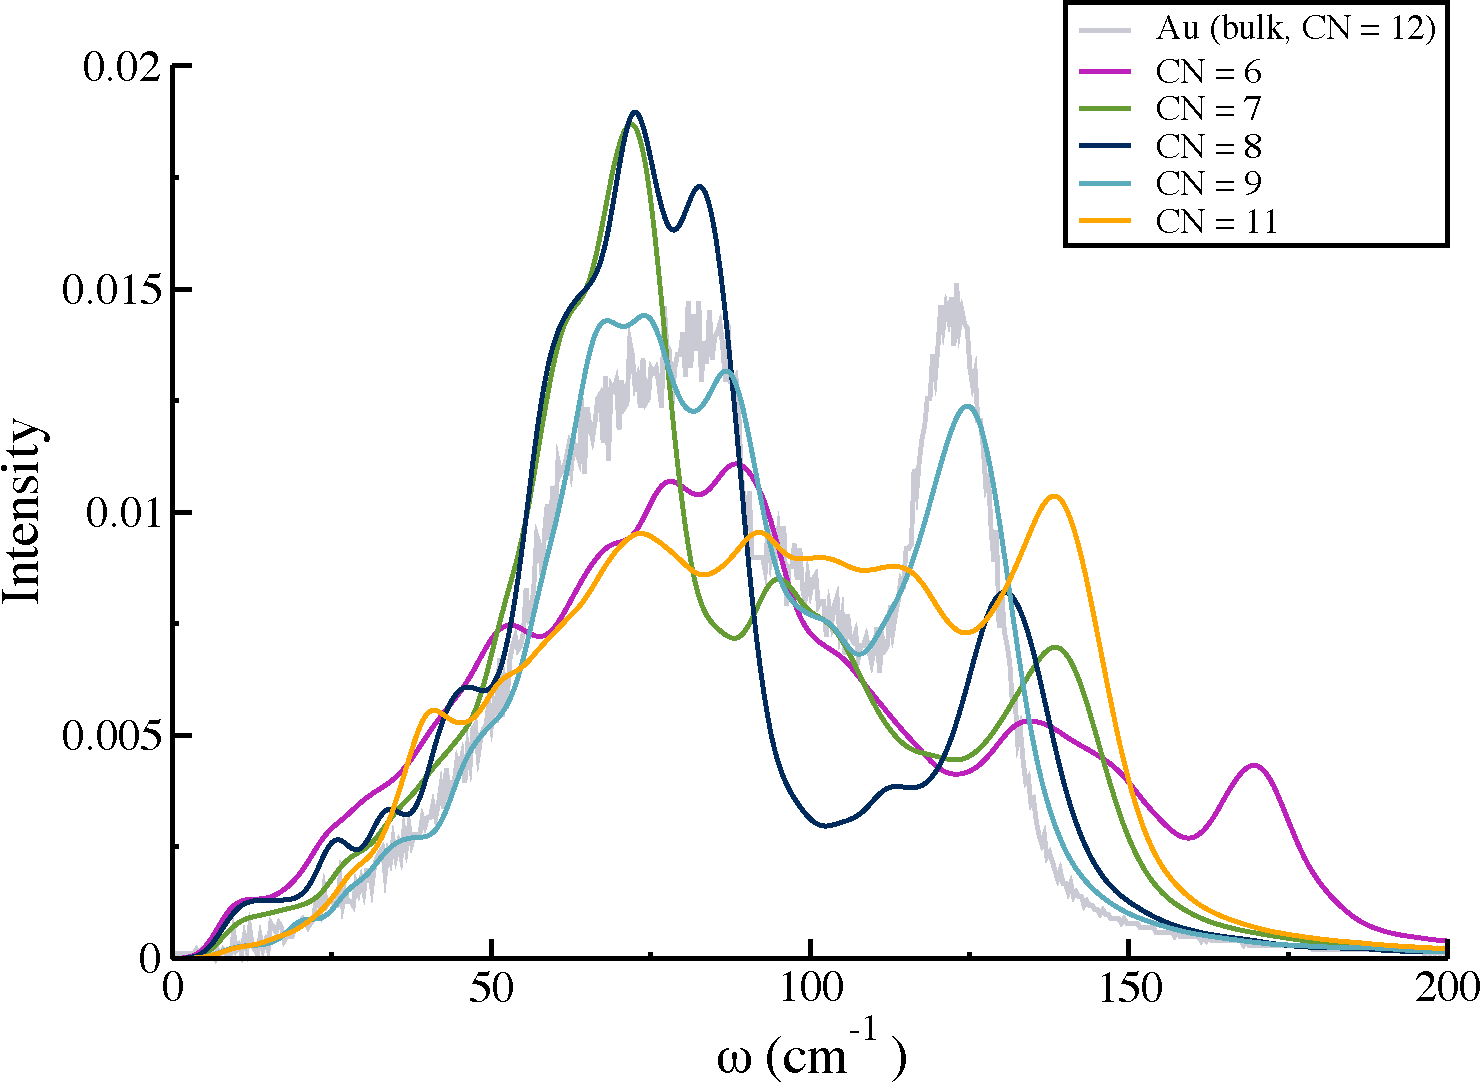
\includegraphics[width=5in]{figures/surface-cn.pdf}
  \caption{The normalized low frequency density of states (DOS) of the
    surface atoms with the coordination number of 6, 7, 8, 9 and 11,
    corresponding to the vertices of the icosahedra, Au(110), Au(100),
    Au(111) and subsurface Au(110), respectively.  Note that CN=11
    atoms near a surface are found adjacent to atoms with lower
    coordination (e.g. CN=7), so the high frequency peak at 138
    cm$^{-1}$ is present for both CN=11 and CN=7.  Low frequency
    contributions at $\sim$ 70 cm$^{-1}$ are enhanced for surface
    atoms with CN=7, 8, and 9.}
  \label{fig:cn-spect}
\end{figure}

Around $\sim$ 70 cm$^{-1}$, the significantly undercoordinated surface
atoms (CN=7,8,9) enhance lower frequency contributions relative to the
bulk.  Simultaneously, the undercoordinated atoms (CN=6,7,8,9) shift
the high frequency peak relative to the bulk at frequencies above
$\sim$ 120 cm$^{-1}$.  The behavior of subsurface (110) atoms with
CN=11 require a bit of explanation. Although many transient CN=11
atoms exist in liquid and bulk configurations, surface environments
that produce CN=11 are tied to nearby lower coordination atoms.  For
(110) surfaces, this is reflected in the VDOS by comparing the peak at
138 cm$^{-1}$ CN=11 and CN=7 atoms.  We conclude that the (110)
surface and subsurface atoms are both involved in phonons with this
frequency.

There is an observed interfacial effect on the vibrational density of
states for the solvent in this system.  Bulk solvent has contributions
from many low-frequency collective motions, while solvent sampled near
the particle interface exhibits collective motions at significantly
higher frequencies. This effect is shown in
Fig. \ref{fig:hexane-comp}.

\begin{figure}[!htb]
	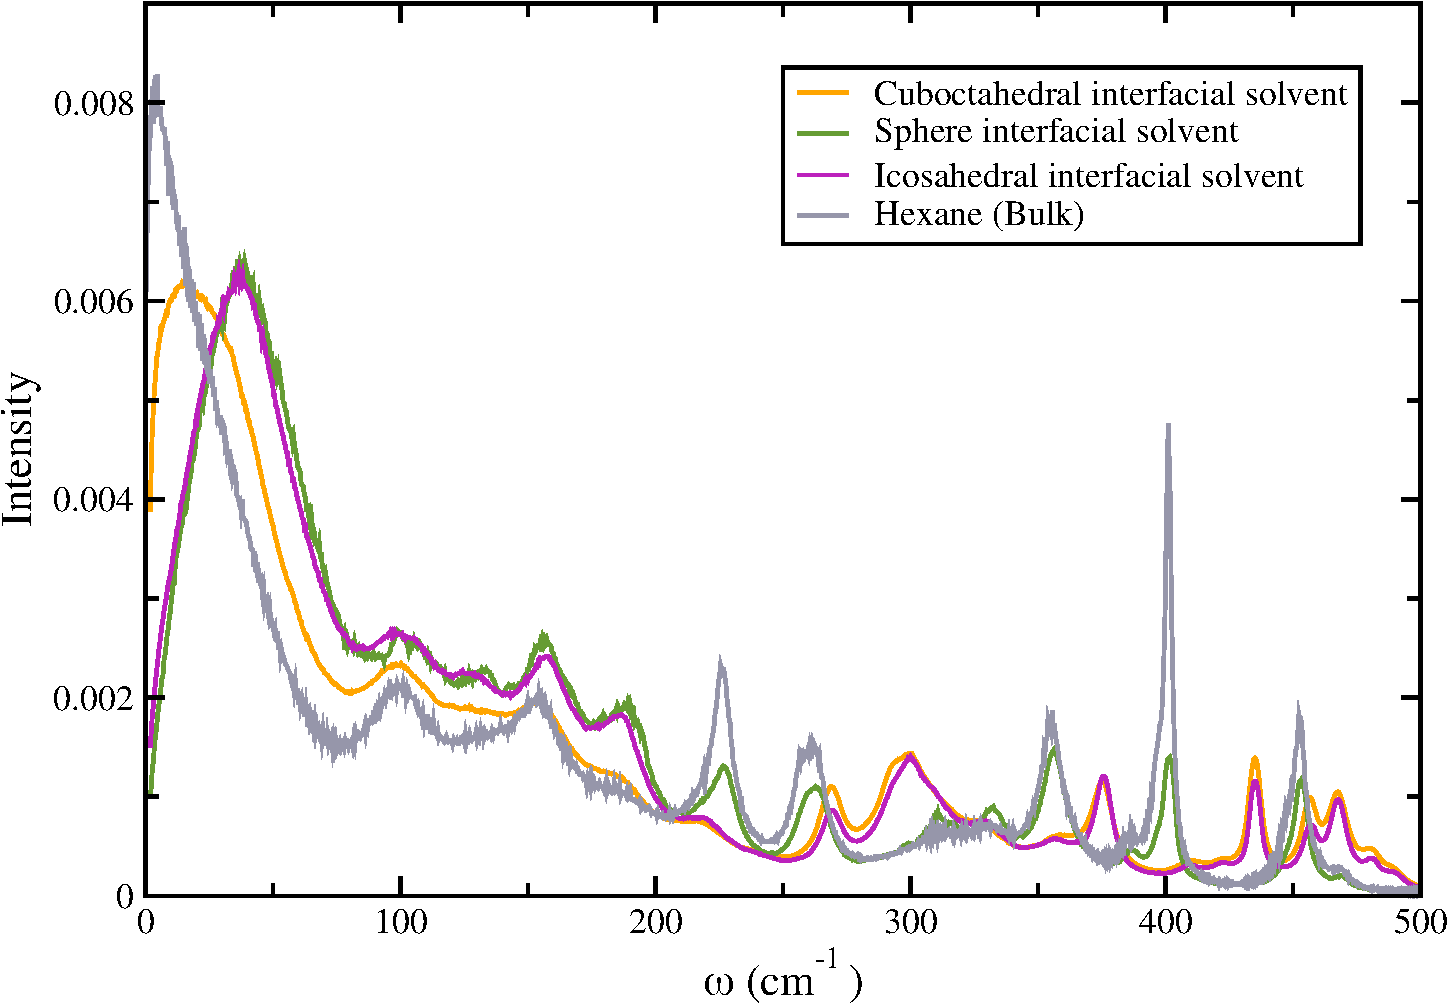
\includegraphics[width=5in]{figures/hexane-comp.pdf}
	\caption{The vibrational density of states (VDOS) for the
          interfacial solvent in the spherical, icosahedral, and
          cuboctahedral systems along with bulk solvent.}
	\label{fig:hexane-comp}
\end{figure}

% \subsection{Phonon transmission at flat interfaces}

% In the main text, we describe a frequency-dependent transmission model, 
% \begin{equation}
% \tau_{a \rightarrow b}(\omega) = \frac{v_b \rho^\perp_b(\omega)}{v_a \rho^\perp_a(\omega) + v_b \rho^\perp_b(\omega)}
% \label{eq:transmission}
% \end{equation}
% and here we present this model's predictions (see
% Fig. \ref{fig:facet-tran}) for the planar facets.  Note that in the
% planar facets, the velocity autocorrelation function is computed using
% only the $z$-axis component in order to project into the interface normal.

% \begin{figure}[!htb]
% 	\includegraphics[width=5in]{figures/facet-tran.pdf}
% 	\caption{The same transmission model described in the main
%           paper, but applied to the three flat facets. Below
%           $25 \text{~cm}^{-1}$ there are significant differences in the
%           transmission probability. The (100) surface, with the
%           highest interfacial thermal conductance, has a highest
%           transmission probability at low frequencies. The surface
%           with the lowest thermal conductance, (111), also has the
%           lowest transmission.} 
%  	\label{fig:facet-tran}
%  \end{figure}

\subsection{Local FCC ordering inside the particles}
One of the observations in the main text is that spheres recover
bulk-like densities of states relatively close to the surface, while
the icosahedra have significantly altered DOS even four layers in to
the particle. Because the icosahedra are constructed around a core
with icosahedral ($\mathrm{I}_h$) symmetry, the local orientational
ordering of atoms deviates from perfect FCC ordering.

We use the fraction of gold atoms exhibiting local fcc ordering as a
function of radius to investigate this effect.  The local bond
orientational order can be described using the method of Steinhardt
\textit{et al.}\cite{Steinhardt1983} The local bonding environment,
$\bar{q}_{\ell m}$, for each atom in the system is determined by
averaging over the spherical harmonics between that atom and each of
its neighbors,
\begin{equation}
\bar{q}_{\ell m} = \sum_i Y_\ell^m(\theta_i, \phi_i)
\end{equation}
where $\theta_i$ and $\phi_i$ are the relative angular coordinates of
neighbor $i$ in the laboratory frame.  A global average orientational
bond order parameter, $\bar{Q}_{\ell m}$, is the average over each
$\bar{q}_{\ell m}$ for all atoms in the system. To remove the
dependence on the laboratory coordinate frame, the third order
rotationally invariant combination of $\bar{Q}_{\ell m}$,
$\hat{w}_\ell$, is utilized here.\cite{Steinhardt1983,Vardeman:2008fk}

For $\ell=4$, the ideal face-centered cubic (FCC) local structures
exhibit $\hat{w}_4$ values near -0.159. Because $\hat{w}_4$ exhibits
an extreme value for fcc structures, it is ideal for measuring local
FCC ordering. The spatial distribution of $\hat{w}_4$ local bond
orientational order parameters, $p(\hat{w}_4 , r)$, can provide
information about the location of individual atoms that are central to
local FCC ordering.

The fraction of FCC-ordered gold atoms at a given radius in the
nanoparticle,
\begin{equation}
        f_\mathrm{fcc}(r) = \int_{-\infty}^{w_c} p(\hat{w}_4, r) d \hat{w}_4
\end{equation}
is described by the distribution of the local bond orientational order
parameters, $p(\hat{w}_4, r)$, and $w_c$, a cutoff for the peak
$\hat{w}_4$ value displayed by fcc structures. As in our previous
work,\cite{Stocker2016} $w_c$ value of -0.12 was chosen to isolate the
fcc peak in $\hat{w}_4$.

As shown in Fig. \ref{fig:struct-bowr}, the FCC ordering persists in
the spheres even quite close to the surface, while the icosahedra have
significant populations that deviate from FCC local ordering.  The
cuboctahedra do not have uniform gold population between 30 and 40
\AA, so the fraction of FCC ordering decays starting at 30 \AA.
Although we cannot conclude that this is the cause of the differences
in the VDOS for the icosahedral particles, it is likely that local
ordering in the metal can alter the bulk densities of states.

\begin{figure}[!htb]
	\includegraphics[width=5in]{figures/struct-bowr.pdf}
	\caption{The fraction of FCC-like local environments as a
          function of radius from the center of 40 \AA\ nanoparticles.
          The spheres and cuboctahedra are originally cut from a FCC
          lattice, so the local ordering persists even close to the
          surface.  Icosahedra are constructed as shells surrounding a
          perfectly icosahedral central core of 13 atoms. Non-FCC
          ordering persists throughout these simulations.}
 	\label{fig:struct-bowr}
 \end{figure}

\subsection{Hexane Density}
The hexane density as function of distance from the gold at the
interface of the planar facets is provided in Fig. \ref{fig:dens}. The
solvent in the (111) and (100) systems display similar behavior, while
the solvent near the (110) interface comes closer to the surface
atoms.  In the (110) system, the first layer of hexane is spread out
over a thicker slab in comparison to the other two systems and allows
solvent to come closer to the interfacial atoms.  This is likely due
to the ridges present on this interface.  Within 5 \AA\ of the
interfacial gold layer, the three systems have the same amount of
hexane.

\begin{figure}
        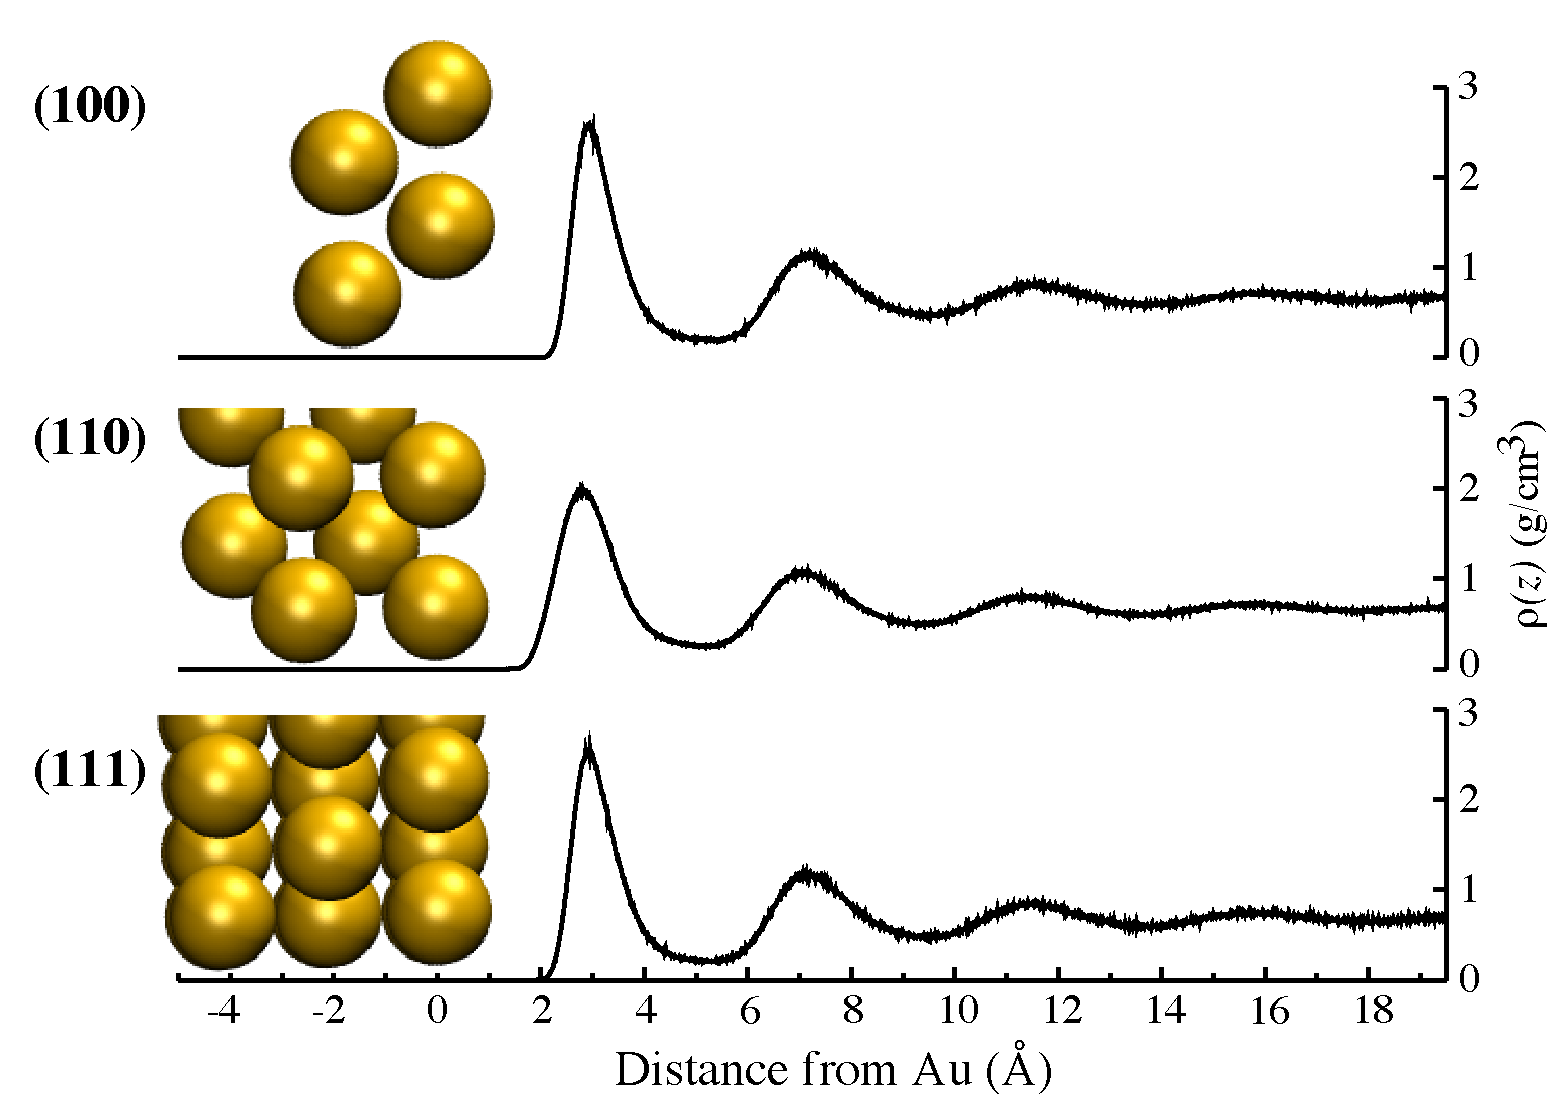
\includegraphics[width=\linewidth]{figures/stacked-hex-facets.pdf}
        \caption{Hexane density as a function of distance from the
          interfacial gold for the (111), (110), and (100) facets. The
          solvent in the (111) and (100) systems display nearly
          identical density profiles. Because the lowest-coordinated
          gold atoms on the (110) facet have a relatively low surface
          density, the hexane molecules are able to get closer to
          these undercoordinated atoms.}
        \label{fig:dens}
\end{figure}

\subsection{A Model for Thermal Conductance}
The model we purpose is a linear combination the surface densities of
undercoordinated atoms, 
\begin{equation}
G \approx a~\mathrm{CN}_{6} + b~\mathrm{CN}_{7} + c~\left(1+c^{\prime}~\delta_\mathrm{ico}\right)~\mathrm{CN}_{8} + d~\left( 1 + d^{\prime}~\delta_\mathrm{ico} \right)~\mathrm{CN}_{9}
\label{eq:lin-fit}
\end{equation}
where, $a - d$ are coordination transport coefficients with the units
of $10^{-20}$ MW/K and $\mathrm{CN}_{n}$ have surface density units
(1/\AA $^2$) for surface atoms with coordination number $n$.  The
delta function, $\delta_\mathrm{ico}$ is set to unity for icosahedral
structures, and zero for FCC-like nanoparticles.  The coefficients
$c^{\prime}$ and $d^{\prime}$ are weighting factors that recognize the
differences in the bulk density of states in the icosahedral
particles. \begin{table}
\centering
\caption{Parameters of the Model in Eq. (\ref{eq:lin-fit}).
  \label{tab:coeff to fit}}
\begin{tabular}{ cccccc }
\toprule
 $a$ & $b$ & $c$ & $c^{\prime}$ & $d$ & $d^{\prime}$ \\
\midrule
 858.9405 & 183.9062 & 291.7960 & -0.5943 & 369.6250 & -0.2498 \\
\bottomrule
\end{tabular}
\end{table}

The coefficients provide some information about the thermal transport
capabilities of each type of undercoordinated surface atom. These fits
suggest that severely undercoordinated atoms (CN=6) transfer the
largest amount of heat per atom, although their population in all
systems is low.

It is also important to note that this fit considers the two different
types of particles when finding the best fits for the most populous
surface atoms (CN=8, CN=9).  If the system is FCC-like the weight of
the CN = 8 and CN = 9 are 2.464 and 1.333 times larger than their
contributions from icosahedral cores.

Since the coefficients are related to the amount of energy transfered
per atom type, these atoms on the FCC-like structures transfer a
larger amount than in the icosahedral structure.  This is likely due
to differences in the underlying ``bulk'' densities of states.

% In Fig. \ref{fig:ideal} the linear fit from Eq. \ref{eq:lin-fit} is
% applied to the ideal particle geometries in Table
% \ref{tab:undercoord}.  The spherical coordination values are taken
% from spheres cut from an FCC lattice without thermal relaxation. The
% fit predicts simliar values for the large icosahedra and cuboctahedra
% as where the simulation values platue, but have an opposite trend in
% the small particles, 10 - 20 \AA.
% \begin{figure}
%         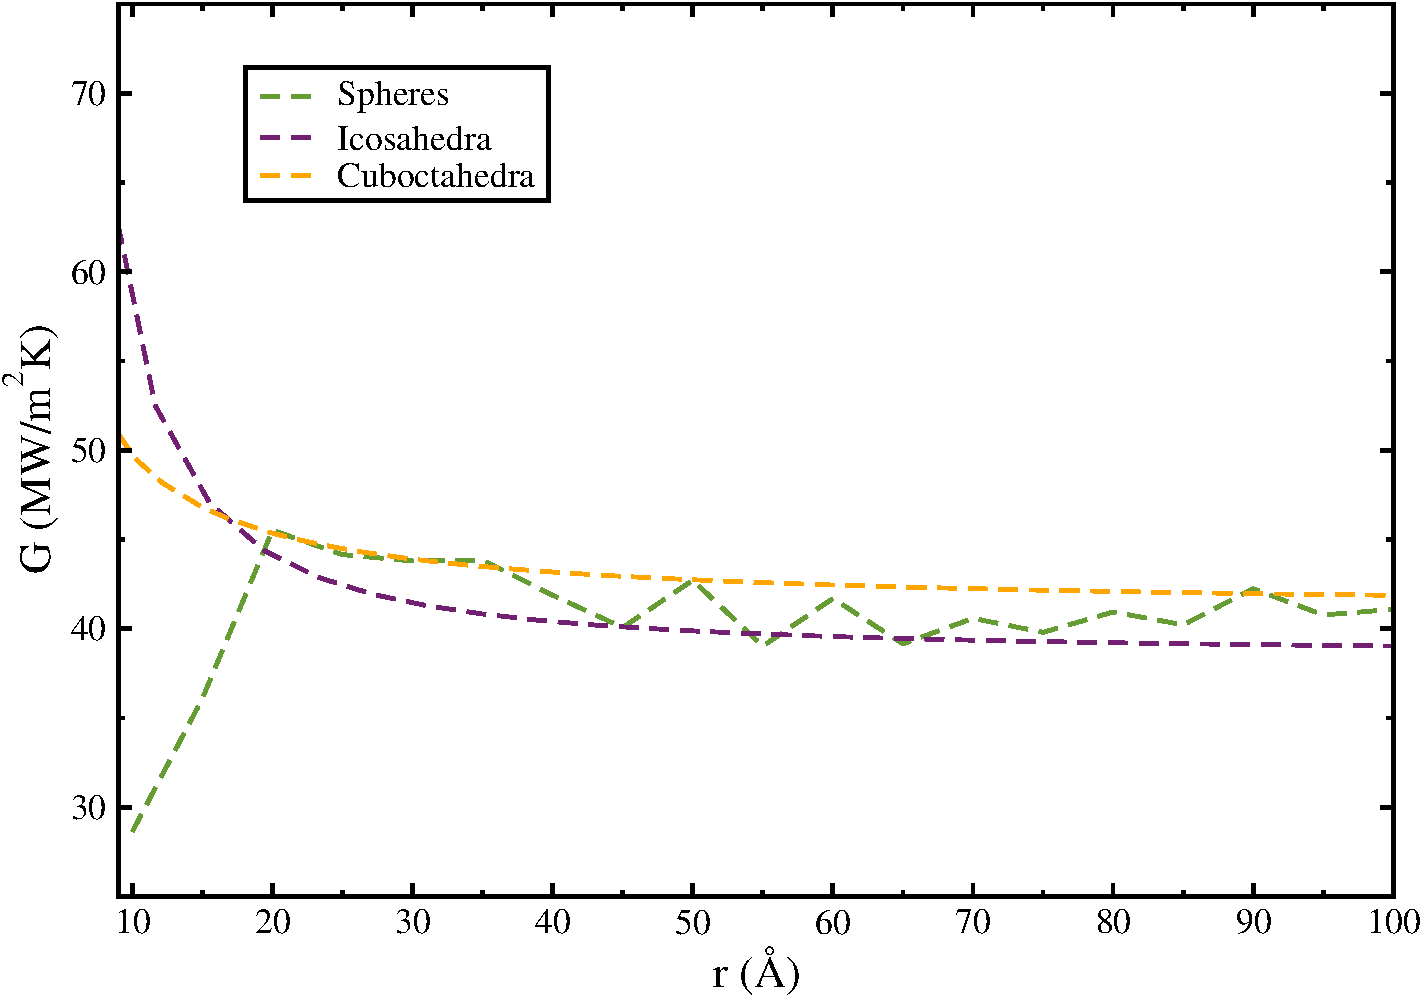
\includegraphics[width=\linewidth]{figures/ideal.pdf}
%         \caption{The interfacial thermal conductance of the ideal geometries for spheres, icosahedra, and cuboctahedra ranging from $\approx$ 10 -- 100 \AA. The icosahedra and cuboctahedra platue to a constant value and have the opposite trend of the simulated systems.} 
%         \label{fig:ideal}
% \end{figure}

\newpage

\bibliography{Morph}

\end{document}
